\chapter{基础理论}
\section{复杂网络和混沌基本理论}
\subsection{图论的基本知识}
记$G=(V,E)$为一个非空图,其中$V$是其顶点集,$E$是边集。图中一点$v$的相邻点集记为$N(v)$,顶点的度是指与其相连的边的个数
记为$d(v)$,一个图的平均度定义为
\begin{equation}
    d(G):=\frac{1}{|V|} \sum_{v \in V} d(v)
\end{equation}
图$G$的一条路径是一个子图,其顶点集与边集描述了原图中某一点到另一点的一条通路。一个圈是指一个子图,描述了以某点为起始点与终止点
的一条非平凡路径。
一个含有$N$个节点、$M$个边的图$G$的密度定义$\rho$为
\begin{equation}
    \rho=\frac{M}{\frac{1}{2} N(N-1)}
\end{equation}
\begin{definition}
    如果非空图$G$中任意两顶点之间均有一条路相连,称图$G$为联通图。
\end{definition}
给定子图 $A,B \subseteq V$ 和 $X \subseteq V \cup E$,如果 $G$ 的每条 $A-B$ 路均包含 $X$ 中的一个顶点或一条边,
称在 $G$ 中 $X$ 分离 (separate) 集合 $A$ 和 $B$ 。
下面是图论中一个重要的定理
\begin{theorem}
    设 $G=(V,E)$ 是一个图且 $A,B \subseteq V$ 。那么,在$G$ 中分离 $A$ 和 $B$ 的顶点的最小数目等于 $G$ 中互不
    相交的 $A-B$ 路的最大数目。
\end{theorem}
\begin{proof}
    对 $\|G\|$ 使用数学归纳法。若 $G$ 不含边,则有 $|A \cap B|=k$ 并且存在 $k$ 条平凡的 $A-B$ 路。 
    设 $G$ 包含边 $e=x y$ 。如果 $G$ 无 $k$ 条不交的 $A-B$ 路,那么 $G / e$ 也没有; 
    若 在 $G$ 中 $x$ 和 $y$ 两顶点中存在一个顶点属于 $A$ (或者 $B$ ),顶点 $v_e$ 
    看为 $G / e$ 中 $A$ (或 者 B) 的元素。由归纳假设,$G / e$ 包含一个少于 $k$ 个顶点的 $A-B$ 分隔 $Y$,
     其中顶点 $v_e$ 在 $Y$ 中; 否则,$Y \subseteq V$ 是 $G$ 的一个 $A-B$ 分隔,矛盾。于是,
     $X:=\left(Y /\left\{v_e\right\}\right) \cup\{x,y\}$ 是 $G$ 的一个 恰好有 $k$ 个顶点的 $A-B$ 分隔。
      所以这个 $A-X$ 分隔至少有 $k$ 个顶点。由归纳假设,$G-e$ 中存在 $k$ 条不交的 $A-X$ 路; 
      同样 $G-e$ 中存在 $k$ 条不交的 $X-B$ 路。由于 $X$ 分离 $A$ 和 $B$,这两个路系统不会在 $G/ X$ 相交,
      故它们可以合并成 $k$ 条不交的 $A-B$ 路。
\end{proof}
网络中节点的距离定义为连接这两个点的最小所经边数目。网络的平均长度定义为
\begin{equation}
    L=\frac{1}{\frac{1}{2} N(N-1)} \sum_{i \neq j} d_{i j}
\end{equation}
其中$d_{ij}$为节点$i,j$之间的距离。如果图本身并不联通,则只计算相连两点的距离的算术平均数。
一个图的直径$D$定义为任意两个节点之间距离的最大值。
\begin{definition}
    图中一个节点$i$的聚类系数$C_i$定义为
\begin{equation}
    C_i=\frac{E_i}{\left(k_i\left(k_i-1\right)\right) / 2}=\frac{2 E_i}{k_i\left(k_i-1\right)}
\end{equation}
其中$k_i$为该节点的度,$E_i$为其$k_i$个邻节点之间存在的边的数目。
还有一种聚类系数的几何定义,两个定义并不等价,一般会加以说明
\begin{equation}
    C_i=\frac{\text { 包含节点 } i \text { 的三角形的数目 }}{\text { 以节点 } i \text { 为中心的连通三元组的数目 }}
\end{equation}
\end{definition}
图的聚类系数定义为节点的聚类系数的均值
\begin{equation}
    C=\frac{1}{N} \sum_{i=1}^N C_i
\end{equation}
\subsection{复杂网络}
复杂网络是指不规则、度分布不均匀的网络模型,生成复杂网络的做法是在规则网络上做具有一定随机性的更改。本节内容会给出
几种常见的复杂网络模型与其性质。
\subsubsection*{ER随机图}
ER随机图是通过给顶点随机连边,这是随机性最强的图。\par
\noindent 具有固定边数的ER 随机图 $G(N,M)$ 构造算法\par
\noindent(1) 初始化: 给定 $N$ 个节点和待添加的边数 $M$ 。\par
\noindent(2) 随机连边:\par
【1】 随机选取一对没有边相连的不同的节点,并在这对节点之间添加一 条边。\par
【2】重复步骤【1】,直至在 $M$ 对不同的节点对之间各添加了一条边。\par
\noindent 以一定概率连接的ER 随机图 $G(N,p)$ 构造算法\par
\noindent(1) 初始化: 给定 $N$ 个节点以及连边概率 $p \in[0,1]$ 。\par
\noindent(2) 随机连边:\par
【1】 选择一对没有边相连的不同的节点。\par
【2】 生成一个随机数 $r \in(0,1)$ 。\par
【3】 如果 $r<p$,那么在这对节点之间添加一条边; 否则就不添加边。\par
【4】 重复步骤【1】-【3】,直至所有的节点对都被选择过一次。\par
主要对第二种$G(N,M)$进行性质分析。首先生成的随机图恰好具有 $M$ 条边的概率为
\begin{equation}
    P(M)=\left(\begin{array}{c}
    C^2_N \\
    M
    \end{array}\right) p^M(1-p)\left(\begin{array}{c}
    N \\
    2
    \end{array}\right)^{-M}
\end{equation}
其中,$C^2_N=\left(\begin{array}{c}
    N \\
    2
    \end{array}\right)$,
$\left(\begin{array}{c}
    C^2_N \\
    M
    \end{array}\right)$表示具有 $N$ 个节点和 $M$ 条边的简单图的数量,
    $p^M(1-p)^{C^2_N-M}$ 
表示有 $M$ 对节点之间添加了边, $C^2_N-M$ 对节点之间没有添加边。
边数分布的平均值为:
\begin{equation}
    \langle M\rangle=\sum_{n=0}^{C^2_N} M P(M)=\left(\begin{array}{l}
    N \\
    2
    \end{array}\right) p=p \frac{N(N-1)}{2}
    \end{equation}
边数分布的方差:
\begin{equation}
    \sigma_M^2=\left\langle M^2\right\rangle-\langle M\rangle^2=p(1-p) \frac{N(N-1)}{2}
\end{equation}
$G(N,M)$中节点度的概率分布符合泊松分布。
\begin{equation}
    P(k)=\left(\begin{array}{c}
    N-1 \\
    k
    \end{array}\right) p^k(1-p)^{N-1-k}
\end{equation}
根据概率统计中的内容,其期望与方差分别为
\begin{equation}
    \langle k\rangle=p(N-1)
\end{equation}
\begin{equation}
    \sigma_k^2=p(1-p)(N-1)
\end{equation}
由于两个节点之间不论是否具有共同的邻居节点,共连接概率均为$p$,所以聚类系数为
\begin{equation}
    C=p=\langle k\rangle /(N-1)
\end{equation}
\subsubsection*{WS小世界模型}
WS小世界模型是通过在规则图上做带有随机性的更改形成的。\par
\noindent WS模型构建算法\par
\noindent(1) 从规则图开始: 给定一个含有 $N$ 个点的环状最近邻耦合网络,其中 每个节点都与它左右相邻的各 $K / 2$ 个节点相连,$K$ 是偶数。\par
\noindent(2) 随机化重连: 以概率 $p$ 随机地重新连接网络中原有的每条边,即把 每条边的一个端点保持不变,另一个端点改取为网络中随机选择的一个节点。
其中规定不得有重边和自环。\par
\begin{figure}[!htbp]
    \centering
    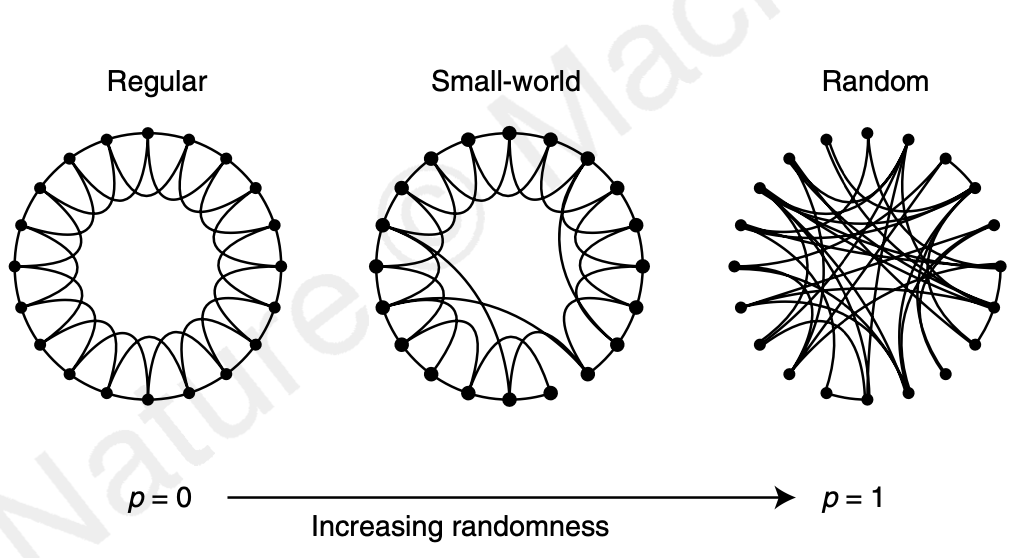
\includegraphics[width=0.8\textwidth]{wsp.png}
\end{figure}
可以看出,$p=0$时是完全规则的网络,$p=1$时是完全随机的网络。WS模型的聚类系数与平均路径长度时关于重连概率$p$的函数
其关系如图
\begin{figure}[!htbp]
    \centering
    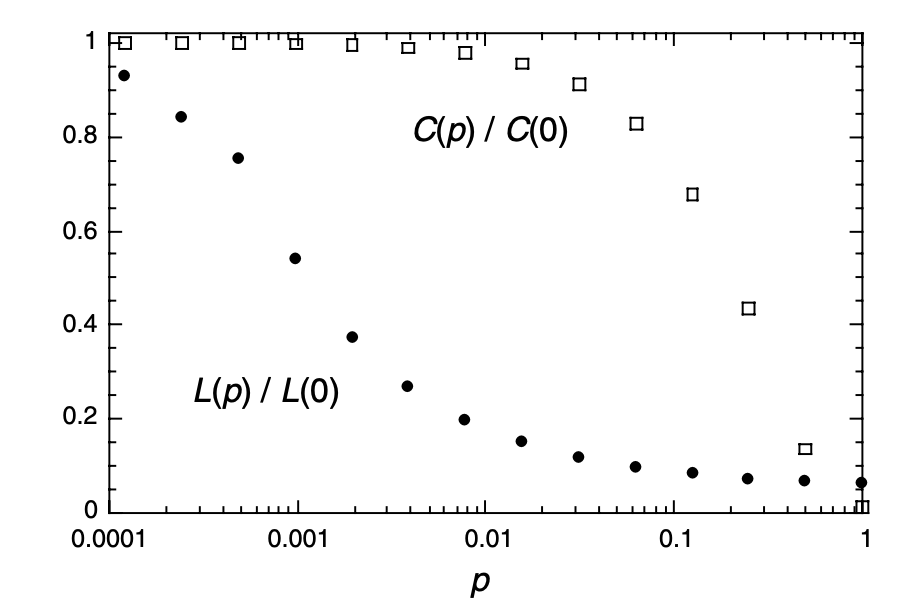
\includegraphics[width=0.8\textwidth]{WS.png}
\end{figure}
WS模型的聚类系数的估计如下
\begin{equation}
    \begin{aligned}
    \tilde{C}_{W S}(p) & \triangleq \frac{M_0(1-p)^3+O(1 / N)}{K(K-1) / 2} \\
    & =\frac{3 K(K-2) / 8}{K(K-1) / 2}(1-p)^3+O(1 / N) \\
    & =\frac{3(K-2)}{4(K-1)}(1-p)^3+O(1 / N) \\
    & =C_{n c}(1-p)^3+O(1 / N)
    \end{aligned}
\end{equation}
下面来研究WS模型的度分布,在 $p>0$ 时,每个节点仍与顺时针方向的 $K / 2$ 条原有的边相连,即每个节点的度至少为 $K / 2$ 。
 为此,记节点 $i$ 的度为 $k_i=s_i+K / 2$。 $s_i$ 又可分为两部分: 
 $s_i=s_i^1+s_i^2,s_i^1$ 表示在原有的与节点 $i$ 相连的逆时针方向的 $K / 2$ 条边中保持不变的边的数目,
 其中每条边不变的概率为 $1-p ; s_i^2$ 表示通过随机重连机制连接节点 $i$ 上的长程边,
 每条这样的边的概率 为 $p / N$ 。有
 \begin{equation}
    \begin{gathered}
    P_1\left(s_i^1\right)=\left(\begin{array}{c}
    K / 2 \\
    s_i^1
    \end{array}\right)(1-p)^{s_i^{1}} p^{K / 2-s_i^1}\\
    P_2\left(s_i^2\right) \simeq \frac{(p K / 2)^{s_i^2}}{\left(s_i^2\right) !} \mathrm{e}^{-\rho K / 2}\text { 当 } N \text { 充分大时. }
    \end{gathered}
\end{equation}
对于任一度为 $k \geqslant K / 2$ 的节点,$s_i^1 \in[0,\min (k-K / 2,K / 2)]$ 。
当$k<K/2$时,$P(k)=0$,当 $k \geqslant$ $K / 2$ 时
\begin{equation}
    P(k)=\sum_{n=0}^{\min (k-K / 2,K / 2)}\left(\begin{array}{c}
    K / 2 \\
    n
    \end{array}\right)(1-p)^n p^{K / 2-n} \frac{(p K / 2)^{k-(K / 2)-n}}{(k-(K / 2)-n) !} \mathrm{e}^{-p K / 2}
\end{equation}
\subsubsection*{NW小世界模型}
NW小世界模型是通过在规则图上做带有随机性的增加长程边形成的,相比WS模型,这是一种更常见的小世界模型。\par
\noindent NW模型构建算法\par
\noindent(1) 从规则图开始: 给定一个含有 $N$ 个节点的环状最近邻耦合网络,其中每个节点都与它左右相邻的各 $K / 2$ 个节点相连,$K$ 是偶数。\par
\noindent(2) 随机化加边: 以概率 $p$ 在随机选取的 $NK / 2$ 对节点之间添加边,其中 规定不得有重边和自环。\par
首先讨论聚类系数,NW模型的聚类系数采用几何聚类系数来讨论,$p=0$ 时,网络中的三角形数量为 
$\frac{1}{4} N K\left(\frac{1}{2} K-1\right)$。$ p>0$ 时,
现在我们需要计算在添加了长程边之后新增加的三角形的数量。 网络中长程边的平均数为 $\frac{1}{2} N K p$,
这些边可以在 $\frac{1}{2} N(N-1)$ 个点对之间添加,每一对节点之间有长程边相连的概率为
\begin{equation}
    \frac{\frac{1}{2} N K p}{\frac{1}{2} N(N-1)}=\frac{K p}{N-1} \approx \frac{K p}{N}
 \end{equation}
 包含一条长程边的三角形数量可以近似为一个与$N$无关的常数:
 \begin{equation}
    N \times \frac{K p}{N}=K p
\end{equation}
当网络规模趋于无穷时,这一常数与最近邻网络的三角形数量相比是可以忽略不计的。因此,对于 $0 \leqslant p \ll 1$ 
模型中的三角形的数量近似为 $\frac{1}{4} N K\left(\frac{1}{2} K-1\right) $
每条长程边都可以与$N$条边的两个端点之一形成连通三元组,因此包含一条长程边的连通三元组的平均数量为
\begin{equation}
    \frac{1}{2} N K p \times K \times 2=N K^2 p
\end{equation}
如果一个节点与 $m>1$ 条长程边相连,那么从中任选两条长程边就构成一个 连通三元组,共有 $\frac{1}{2} m(m-1)$ 种可能。
平均一个节点与 $K p$ 条长程边相连,因此 网络中以一个节点为中心的包含两条长程边的连通三元组数量的均值为
\begin{equation}
    N \times \frac{1}{2} K p(K p-1) \approx \frac{1}{2} N K^2 p^2
\end{equation}
因此,NW模型中总的连通三元组的数量的均值为
\begin{equation}
    \frac{1}{2} N K(K-1)+N K^2 p+\frac{1}{2} N K^2 p^2
\end{equation}
综上所述,当$0 \leqslant p<1$时,NW小世界网络模型的聚类系数的估计值为
\begin{equation}
    \begin{aligned}
    \tilde{C}_{N W}(p) & =\frac{3 \times \frac{1}{4} N K\left(\frac{1}{2} K-1\right)}{\frac{1}{2} N K(K-1)+N K^2 p+\frac{1}{2} N K^2 p^2} \\
    & =\frac{3(K-2)}{4(K-1)+4 K p(p+2)} 
    \end{aligned}
\end{equation}
小世界模型的平均路径长度具有如下形式
\begin{equation}
    L=\frac{N}{K} f(N K p)
\end{equation}
$f(x)$被称为普适标度函数,NW模型的平均路径长度有如下近似
\begin{equation}
    f(x)=\frac{2}{\sqrt{x^2+4 x}} \operatorname{artanh} \sqrt{\frac{x}{x+4}}
\end{equation}
在$x$远大于1时,可以简化为
\begin{equation}
    f(x) \simeq \frac{1}{\sqrt{x^2+4 x}} \ln \frac{\sqrt{1+4 / x}+1}{\sqrt{1+4 / x}-1} \simeq \frac{\ln x}{x},\quad x>>1
\end{equation}
将$f(x)$代入,最后得出
\begin{equation}
    L=\frac{\ln (N K p)}{K^2 p},\quad N K p>>1
\end{equation}
由图看出,这种近似效果优异。\par
\begin{figure}[!htbp]
    \centering
    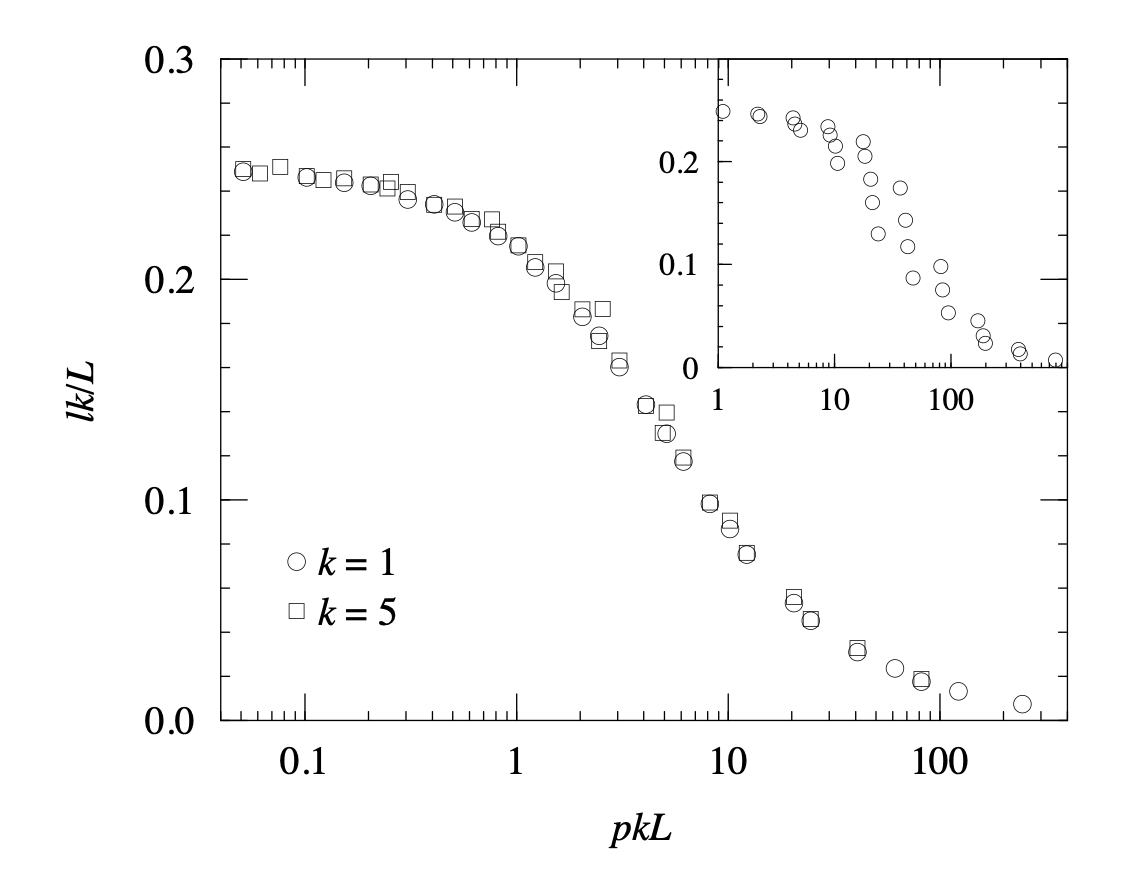
\includegraphics[width=0.8\textwidth]{NW1.png}
\end{figure}
下面讨论度分布,由于每对节点之间有边相连的概率为 $Kp/(N-1)$,因此
\begin{equation}
    P(k)=\left(\begin{array}{l}
    N-1 \\
    k-K
    \end{array}\right)\left[\frac{K p}{N-1}\right]^{k-K}\left[1-\frac{K p}{N-1}\right]^{N-1-k+K}
\end{equation}
NW模型中长程边的平均数为 $\frac{1}{2} N K p$,涉及的端点数目为 $N K p$ 。
因此,网络中长程边的数量为 $K p$,
即 $\langle k-K\rangle=K p$ 。当网络中节点数 $N$ 充分大时,可近似写为泊松分布:
\begin{equation}
    P(k)=\frac{(K p)^{k-K}}{(k-K) !} \mathrm{e}^{-K_p}
\end{equation}
\subsection{混沌}
在刘慈欣的著作《三体》中提到了一个经典的天体物理问题——三体问题,这个问题的一个重要特点是三体系统的不稳定性,即在微小扰动的影响下,
依托于一定时间内已知的位置与运动信息预测出将来的位置具有很大的变化。现实中很难把握系统中全部的微信息,例如一个原子的微小扰动几乎是
难以描述的,如果模型自身对这种微小差异敏感度极高,那意味着这个系统几乎没有可以预测的可能性,预测出的结果与现实差异会随着时间轴指数级放大。
衡量非线性系统的稳定性研究主要由李雅普诺夫稳定性入手,首先来研究系统自身的稳定性。
考虑自治系统
\begin{equation}
    \dot{x}=f(x)
\end{equation}
其中 $,f: D \rightarrow R^n$ 是从定义域 $D \subset R^n$ 到 $R^n$ 上的局部利普希茨映射。
假定 $\bar{x} \in D$ 是其平衡点,即 $f(\bar{x})=0$ 。不失一般性,所有定义和定理都是对平衡点在 $R^n$ 上的原点,
即 $\bar{x}=0$ 时的情况而言。因为经过变量代换总可以把平衡点变换为原点。假设 $\bar{x} \neq 0$,经 $y=x-\bar{x}$ 变换后,$y$ 的
导数为
\begin{equation}
    \dot{y}=\dot{x}=f(x)=f(y+\bar{x}) \stackrel{\text { def }}{=} g(y),g(0)=0
\end{equation}
对于变量$y$,系统在原点有平衡点。
\begin{definition}
    对于平衡点$x=0$,如果对于每个 $\varepsilon>0$,都存在 $\delta=\delta(\varepsilon)>0$, 满足
    \begin{equation}
        \|x(0)\|<\delta \Rightarrow\|x(t)\|<\varepsilon,\quad \forall t \geqslant 0
    \end{equation}
    则该平衡,点是稳定的。
    如果稳定,且可选择适当的 $\delta$, 满足
    \begin{equation}
        \|x(0)\|<\delta \Rightarrow \lim _{t \rightarrow \infty} x(t)=0
    \end{equation}
    则该平衡,点是渐近稳定的。
\end{definition}
下面的李雅普诺夫稳定性定理是判断平衡点稳定的重要方法,它能够用某些其他函数代替能量以确定平衡点的稳定性。
设 $V: D \rightarrow R$ 是连续可微函数,$\dot{V}(x)$是$V(x)$沿方程轨线的导数。即
\begin{equation}
    \begin{aligned}
    \dot{V}(x) & =\sum_{i=1}^n \frac{\partial V}{\partial x_i} \dot{x}_i=\sum_{i=1}^n \frac{\partial V}{\partial x_i} f_i(x) \\
    & =\left[\begin{array}{llll}
    \frac{\partial V}{\partial x_1},& \frac{\partial V}{\partial x_2},& \cdots,& \frac{\partial V}{\partial x_n}
    \end{array}\right]\left[\begin{array}{c}
    f_1(x) \\
    f_2(x) \\
    \vdots \\
    f_n(x)
    \end{array}\right]=\frac{\partial V}{\partial x} f(x)
    \end{aligned}
\end{equation}
\begin{theorem}
    设 $x=0$ 是方程的一个平衡点,$D \subset R^n$ 是包含原点的定义域。设 $V: D \rightarrow R$ 是连续可微函数,如果
    \begin{equation}
        \begin{array}{lll}
        V(0)=0,& V(x)>0 & \text { 在 } D-\{0\} \text { 内 } \\
        & \dot{V}(x) \leqslant 0 & \text { 在 } D \text { 内 }
        \end{array}
    \end{equation}
    那么,原点 $x=0$ 是稳定的。此外,如果
    \begin{equation}
        \dot{V}(x)<0 \quad \text { 在 } D-\{0\} \text { 内 }
    \end{equation}
    那么,原点 $x=0$ 是渐近稳定的。
\end{theorem}
\begin{proof}
    给定 $\varepsilon>0$,任意 $r \in(0,\varepsilon]$,有
    \begin{equation}
        B_r=\left\{x \in R^n \mid\|x\| \leqslant r\right\} \subset D
    \end{equation}
    设 $\alpha=\min _{\|x\|=r} V(x)$,则由式 (2.33) 得 $\alpha>0$ 。取 $\beta \in(0,\alpha)$,设
    \begin{equation}
        \Omega_\beta=\left\{x \in B_r \mid V(x) \leqslant \beta\right\}
    \end{equation}
    那么,$\Omega_\beta$ 在 $B_r$ 内  。集合 $\Omega_\beta$ 有如下的性质,
    当 $t \geqslant 0$ 时,在 $t=0$ 时刻始于 $\Omega_\beta$ 内的任何轨线都保持在 $\Omega_\beta$ 内, 因为
    \begin{equation}
        \dot{V}(x(t)) \leqslant 0 \Rightarrow V(x(t)) \leqslant V(x(0)) \leqslant \beta,\forall t \geqslant 0
    \end{equation}
    由于 $\Omega_\beta$ 是紧集,只要 $x(0) \in \Omega_\beta$,则对于所有 $t \geqslant 0$,方程有唯一解。
    因为 $V(x)$ 连续且 $V(0)=0$,故存在 $\delta>0$ 满足
    \begin{equation}
        \|x\| \leqslant \delta \Rightarrow V(x)<\beta
    \end{equation}
    那么
    \begin{equation}
        B_\delta \subset \Omega_\beta \subset B_r
    \end{equation}
    并且
    \begin{equation}
        x(0) \in B_\delta \Rightarrow x(0) \in \Omega_\beta \Rightarrow x(t) \in \Omega_\beta \Rightarrow x(t) \in B_r
    \end{equation}
    因此
    \begin{equation}
        \|x(0)\|<\delta \Rightarrow\|x(t)\|<r \leqslant \varepsilon,\quad \forall t \geqslant 0
    \end{equation}
    因此平衡点$x=0$是稳定的。现在假设式(2.34)也成立,证明渐近稳定性,即对于每个 $a>0$,存在 $T>0$,使对于所有 $t>T$ 都有 $\|x(t)\|<a$ 。
    由于对于每个 $a>0$,可选择 $b>0$,满足 $\Omega_b \subset B_a$,因此,$t$趋于无穷时,$V(x(t))$趋于零所以有。
    \begin{equation}
        V(x(t)) \rightarrow c \geqslant 0 \text { 当 } t \rightarrow \infty
    \end{equation}
    证明 $c=0$,采用反证法。假设 $c>0$,由 $V(x)$ 的连续性可知,存在 $d>0$ 使 $B_d \subset \Omega_c$ 。
    $V(x(t)) \rightarrow c>0$ 是指所有 $t \geqslant 0$,轨线 $x(t)$ 位于球 $B_d$ 之外。
    设 $-\gamma=\max _{d \leqslant\|x\| \leqslant r} \dot{V}(x)$,因为连续函数 $\dot{V}(x)$ 在紧集 $\{d \leqslant\|x\| \leqslant r\}$ (1) 上有最大值。
    由式 (2.34) 可知,$-\gamma<0$,从 而有
    \begin{equation}
        V(x(t))=V(x(0))+\int_0^t \dot{V}(x(\tau)) d \tau \leqslant V(x(0))-\gamma t
    \end{equation}
    该不等式右项最终为负,故与假设相矛盾。
\end{proof}
满足式(2.33)的连续可微函数 $V(x)$ 称为李雅普诺夫函数。对于某个 $c>0$,曲面 $V(x)=c$ 称为李雅普诺夫面或等位面。
下面是Barbashin-Krasovski定理。 
\begin{theorem}
    设 $x=0$ 是方程的平衡点,$V: R^n \rightarrow R$ 是一个连续可微函数,且满足
    \begin{equation}
        \begin{gathered}
        V(0)=0 \text { 且 } V(x)>0,\quad \forall x \neq 0 \\
        \|x\| \rightarrow \infty \Rightarrow V(x) \rightarrow \infty \\
        \dot{V}(x)<0,\quad \forall x \neq 0
        \end{gathered}
     \end{equation}
\end{theorem}
下面是Chetaev定理,用于确定非稳定平衡点的不稳定性。
\begin{theorem}
    设 $x=0$ 是方程 $(4.1)$ 的平衡点。设 $V: D \rightarrow R$ 是连续可微函数,满足 $V(0)=0$,
    且对于任意小 $\left\|x_0\right\|$ 的某一点 $x_0$,有 $V\left(x_0\right)>0$ 。定义集合 $U=\left\{x \in B_r \mid V(x)>0\right\}$,
    并假设在 $U$ 内有 $\dot{V}(x)>0$,那么 $x=0$ 就是非稳定平衡点。
\end{theorem}
接下来讨论非线性系统线性化的方法,定义线性系统
\begin{equation}
    \dot{x}=A x
\end{equation}
该系统在原点处有一个平衡点,当且仅当 $\operatorname{det}(A) \neq 0$ 时,该平衡点是孤立的。
如果 $\operatorname{det}(A)=0$,则矩阵 $A$ 有一个非平凡零空间。 $A$ 的零空间内的每一点都是系统的平衡点,进而系统有一个平衡点子空间。
线性系统不可能有多个孤立的平衡点, 因为如果 $\bar{x}_1$ 和 $\bar{x}_2$ 是系统的两个平衡点, 那么连接 $\bar{x}_1$ 和 $\bar{x}_2$ 
两点的直线上的每一点都是系统的平衡点。原点的稳定性质由矩阵 $A$ 的特征值位置决定。对于给定的初始状态 $x(0)$,系统的解为
\begin{equation}
    x(t)=\exp (A t) x(0)
\end{equation}
转换为若尔当标准型
\begin{equation}
    P^{-1} A P=J=\text { block } \operatorname{diag}\left[J_1,J_2,\cdots,J_r\right]
\end{equation}
\begin{equation}
    J_i=\left[\begin{array}{cccccc}
    \lambda_i & 1 & 0 & \ldots & \ldots & 0 \\
    0 & \lambda_i & 1 & 0 & \ldots & 0 \\
    \vdots & & \ddots & & & \vdots \\
    \vdots & & & \ddots & & 0 \\
    \vdots & & & & \ddots & 1 \\
    0 & \ldots & \ldots & \ldots & 0 & \lambda_i
    \end{array}\right]_{m \times m}
\end{equation}
因此
\begin{equation}
    \exp (A t)=P \exp (J t) P^{-1}=\sum_{i=1}^r \sum_{k=1}^{m_i} t^{k-1} \exp \left(\lambda_i t\right) R_{i k}
\end{equation}
\begin{theorem}
    当且仅当 $A$ 的所有特征值都满足 $\operatorname{Re} \lambda_i \leqslant 0$,对于每个 $\operatorname{Re} \lambda_i=0$,
    代数重数 $q_i \geqslant 2$ 的特征值满足 $\operatorname{rank}\left(A-\lambda_i I\right)=n-q_i$ 时
    ($n$ 为 $x$ 的维数),方程 $\dot{x}=A x$ 的平衡点 $x=0$ 是稳定的。 
    当且仅当 $A$ 的所有特征值满足 $\operatorname{Re} \lambda_i<0$ 时,平衡点 $x=0$ 是全局渐近稳定的。
\end{theorem}
回到非线性系统(2.29),$f: D \rightarrow R^n$ 是从 $D \subset R^n$ 到 $R^n$ 的连续可微映射。
假设原点 $x=0$ 在 $D$ 内,且为系统的一个 平衡点,即 $f(0)=0$ 。根据均值定理
\begin{equation}
    f_i(x)=f_i(0)+\frac{\partial f_i}{\partial x}\left(z_i\right) x
\end{equation}
其中 $z_i$ 是连接 $x$ 与原点之间的线段上的一点。由于$f(0)=0$
\begin{equation}
    f_i(x)=\frac{\partial f_i}{\partial x}\left(z_i\right) x=\frac{\partial f_i}{\partial x}(0) x+\left[\frac{\partial f_i}{\partial x}\left(z_i\right)-\frac{\partial f_i}{\partial x}(0)\right] x
\end{equation}
所以
\begin{equation}
    f(x)=A x+g(x)
\end{equation}
其中
\begin{equation}
    A=\frac{\partial f}{\partial x}(0),\quad g_i(x)=\left[\frac{\partial f_i}{\partial x}\left(z_i\right)-\frac{\partial f_i}{\partial x}(0)\right] x
\end{equation}
并且
\begin{equation}
    \left|g_i(x)\right| \leqslant\left\|\frac{\partial f_i}{\partial x}\left(z_i\right)-\frac{\partial f_i}{\partial x}(0)\right\|\|x\|
\end{equation}
\begin{equation}
    \frac{\|g(x)\|}{\|x\|} \rightarrow 0 \text {,当 }\|x\| \rightarrow 0
\end{equation}
这就是说在原点的一个小邻域内,可以用对系统在原点的线性化方程
\begin{equation}
    \dot{x}=A x,\quad \text { 其中 } A=\frac{\partial f}{\partial x}(0)
\end{equation}
下面定理指出当原点是非线性系统的平衡点时,其稳定性可以通过研究线性系统在该平衡点的稳定性得出。
\begin{theorem}
    设 $x=0$是非线性系统$\quad \dot{x}=f(x)$的一个平衡点,其中 $f: D \rightarrow R^n$ 是连续可微的,
    且 $D$ 为原点的一个邻域。设
    \begin{equation}
        A=\left.\frac{\partial f}{\partial x}(x)\right|_{x=0}
    \end{equation}
    如果 $A$ 的所有特征值都满足 $\operatorname{Re} \lambda_i<0$,则原点是渐近稳定的。如果 $A$ 至少有一个特征值满足 $\operatorname{Re} \lambda_i>0$,则原点是不稳定的。
\end{theorem}
\begin{proof}
    首先证明第一条,由于任何正定对称矩阵$Q$,李雅普诺夫方程的解$P$都是正定的。令$V(x)=x^{\mathrm{T}} P x$,则
    \begin{equation}
        \begin{aligned}
        \dot{V}(x) & =x^{\mathrm{T}} P f(x)+f^{\mathrm{T}}(x) P x \\
        & =x^{\mathrm{T}} P[A x+g(x)]+\left[x^{\mathrm{T}} A^{\mathrm{T}}+g^{\mathrm{T}}(x)\right] P x \\
        & =x^{\mathrm{T}}\left(P A+A^{\mathrm{T}} P\right) x+2 x^{\mathrm{T}} P g(x) \\
        & =-x^{\mathrm{T}} Q x+2 x^{\mathrm{T}} P g(x)
        \end{aligned}
    \end{equation}
    其中
    \begin{equation}
        \frac{\|g(x)\|_2}{\|x\|_2} \rightarrow 0 \text { 当 }\|x\|_2 \rightarrow 0
    \end{equation}
    对于任意 $\gamma>0$,存在 $r>0$,使
    \begin{equation}
        \|g(x)\|_2<\gamma\|x\|_2,\quad \forall\|x\|_2<r
    \end{equation}
    因此
    \begin{equation}
        \dot{V}(x)<-x^{\mathrm{T}} Q x+2 \gamma\|P\|_2\|x\|_2^2,\quad \forall\|x\|_2<r
    \end{equation}
    但是
    \begin{equation}
        x^{\mathrm{T}} Q x \geqslant \lambda_{\min }(Q)\|x\|_2^2
    \end{equation}
    其中 $\lambda_{\min }(\cdot)$ 表示矩阵的最小特征值。注意, 由于 $Q$ 是对称且正定的,
    所以 $\lambda_{\text {min }}(Q)$ 为正实数,因此
    \begin{equation}
        \dot{V}(x)<-\left[\lambda_{\min }(Q)-2 \gamma\|P\|_2\right]\|x\|_2^2,\quad \forall\|x\|_2<r
    \end{equation}
    选择 $\gamma<(1 / 2) \lambda_{\min }(Q) /\|P\|_2$, 以保证 $\dot{V}(x)$ 负定,
    所以原点是渐近稳定的。\par
    证明定理的第二条,先考虑 $A$ 在虚轴上没有特征值的特例。如果 $A$ 的特征值集中到右半开平面为一组,
    左半开平面为一组,那么存在一个满秩矩阵 $T$, 满足
    \begin{equation}
        T A T^{-1}=\left[\begin{array}{cc}
        -A_1 & 0 \\
        0 & A_2
        \end{array}\right]
    \end{equation}
    并使得$A_1,A_2$的特征值实部均小于零,令
    \begin{equation}
        z=T x=\left[\begin{array}{l}
        z_1 \\
        z_2
        \end{array}\right]
    \end{equation}
    $z$ 的分块与 $A_1$ 和 $A_2$ 的维数一致。进行变量代换 $z=T x$,则系统
    \begin{equation}
        \dot{x}=A x+g(x)
    \end{equation}
    被分解为
    \begin{equation}
        \begin{aligned}
        & \dot{z}_1=-A_1 z_1+g_1(z) \\
        & \dot{z}_2=A_2 z_2+g_2(z)
        \end{aligned}
    \end{equation}
    对于任意 $\gamma>0$,存在$r>0$,对函数 $g_i(z)$ 有
    \begin{equation}
        \left\|g_i(z)\right\|_2<\gamma\|z\|_2, \quad \forall\|z\|_2 \leqslant r, i=1,2
    \end{equation}
    设$Q_1$和$Q_2$分别是$A_1$和$A_2$,维数相同的正定对称短阵。则方程
    \begin{equation}
        P_i A_i+A_i^{\mathrm{T}} P_i=-Q_i, \quad i=1,2
    \end{equation}
    有唯一的正定解 $P_1$ 和 $P_2$ 。设
    \begin{equation}
        V(z)=z_1^{\mathrm{T}} P_1 z_1-z_2^{\mathrm{T}} P_2 z_2=z^{\mathrm{T}}\left[\begin{array}{cc}
        P_1 & 0 \\
        0 & -P_2
        \end{array}\right] z
    \end{equation}
    在子空间 $z_2=0$ 内,对于任意靠近原点的点有 $V(z)>0$ 。设
    \begin{equation}
        U=\left\{z \in R^n \mid\|z\|_2 \leqslant r \text { 和 } V(z)>0\right\}
    \end{equation}
    则在$U$内,有
    \begin{equation}
        \begin{aligned}
        \dot{V}(z)= & -z_1^{\mathrm{T}}\left(P_1 A_1+A_1^{\mathrm{T}} P_1\right) z_1+2 z_1^{\mathrm{T}} P_1 g_1(z) \\
        & -z_2^{\mathrm{T}}\left(P_2 A_2+A_2^{\mathrm{T}} P_2\right) z_2-2 z_2^{\mathrm{T}} P_2 g_2(z) \\
        = & z_1^{\mathrm{T}} Q_1 z_1+z_2^{\mathrm{T}} Q_2 z_2+2 z^{\mathrm{T}}\left[\begin{array}{c}
        P_1 g_1(z) \\
        -P_2 g_2(z)
        \end{array}\right] \\
        \geqslant & \lambda_{\min }\left(Q_1\right)\left\|z_1\right\|_2^2+\lambda_{\min }\left(Q_2\right)\left\|z_2\right\|_2^2 \\
        & -2\|z\|_2 \sqrt{\left\|P_1\right\|_2^2\left\|g_1(z)\right\|_2^2+\left\|P_2\right\|_2^2\left\|g_2(z)\right\|_2^2} \\
        > & (\alpha-2 \sqrt{2} \beta \gamma)\|z\|_2^2
        \end{aligned}
    \end{equation}
    其中
    \begin{equation}
        \alpha=\min \left\{\lambda_{\min }\left(Q_1\right), \lambda_{\min }\left(Q_2\right)\right\}, \quad \beta=\max \left\{\left\|P_1\right\|_2,\left\|P_2\right\|_2\right\}
    \end{equation}
    选择 $\gamma<\alpha /(2 \sqrt{2} \beta)$保证在 $U$ 内有 $\dot{V}(z)>0$ 。所以原点是非稳定的。通过定义矩阵
    \begin{equation}
        P=T^{\mathrm{T}}\left[\begin{array}{cc}
        P_1 & 0 \\
        0 & -P_2
        \end{array}\right] T ; \quad Q=T^{\mathrm{T}}\left[\begin{array}{cc}
        Q_1 & 0 \\
        0 & Q_2
        \end{array}\right] T
    \end{equation}
    满足方程
    \begin{equation}
        P A+A^{\mathrm{T}} P=Q
    \end{equation}
    矩阵 $Q$ 是正定的,并且 $V(x)=x^{\mathrm{T}} P x$ 在任意靠近原点 $x=0$ 点上为正。
    现在考虑 $A$ 在虚轴上可能有特征值,而且在右半开复平面内也有特征值。
    运用平移坐标轴的简单方法,将一般情况转化为特殊情况。假设 $A$ 有 $m$ 个特征值,
    且满足 $\operatorname{Re} \lambda_i>\delta>0$ 。那么,矩 阵 $[A-(\delta / 2) I]$ 在右半开平面内有 $m$ 个特征值,
    但在虚轴上没有特征值。存在矩阵 $P=P^{\mathrm{T}}$ 和 $Q=Q^{\mathrm{T}}>0$,使
    \begin{equation}
        P\left[A-\frac{\delta}{2} I\right]+\left[A-\frac{\delta}{2} I\right]^{\mathrm{T}} P=Q
    \end{equation}
    其中,$V(x)=x^{\mathrm{T}} P x$ 对任意靠近原点的点都为正,则
    \begin{equation}
        \begin{aligned}
        \dot{V}(x) & =x^{\mathrm{T}}\left(P A+A^{\mathrm{T}} P\right) x+2 x^{\mathrm{T}} P g(x) \\
        & =x^{\mathrm{T}}\left[P\left(A-\frac{\delta}{2} I\right)+\left(A-\frac{\delta}{2} I\right)^{\mathrm{T}} P\right] x+\delta x^{\mathrm{T}} P x+2 x^{\mathrm{T}} P g(x) \\
        & =x^{\mathrm{T}} Q x+\delta V(x)+2 x^{\mathrm{T}} P g(x)
        \end{aligned}
    \end{equation}
    在集合$\left\{x \in R^n \mid\|x\|_2 \leqslant r\right.$ 且 $\left.V(x)>0\right\}$内,当 $\|x\|_2<r$ 时,选择 $r$ 满足 $\|g(x)\|_2 \leqslant \gamma\|x\|_2$,
    则 $\dot{V}(x)$ 满足
    \begin{equation}
        \dot{V}(x) \geqslant \lambda_{\min }(Q)\|x\|_2^2-2\|P\|_2\|x\|_2\|g(x)\|_2 \geqslant\left(\lambda_{\min }(Q)-2 \gamma\|P\|_2\right)\|x\|_2^2
    \end{equation}
    当 $\gamma<(1 / 2) \lambda_{\text {min }}(Q) /\|P\|_2$ 时,上式为正,运用Chetaev 定理(定理2.4)即可证明。
\end{proof}

\section{稀疏重构基本理论和算法}
\subsection{稀疏重构基本理论}
该节介绍了压缩感知理论的定义以及基础数学知识,通过探寻不同的限制与不同的感应矩阵性质给出稀疏重构问题解的唯一性与存在性
的等价条件。如若未说明,本节内容只讨论实向量空间,可拓展至复数的会单独指明。
\subsubsection{稀疏重构问题的定义}
假设信号$x=\left(x_i\right)^n_{i=1}\in \mathbb{R}^n$具有稀疏性质,或者在一个正交变换后具有这样的性质即
$\Vert x\Vert_0:=\# \{i:x_i \neq 0\}$远小于$n$或$x=\Phi c$,$\Phi$是正交矩阵且$c$稀疏。
取$m\times n$的矩阵$A$,其中$m<n$。令
\begin{equation}
    y=Ax,y=A\Phi c
\end{equation}
稀疏重构问题是指在已知原向量$x$中零元素足够多的情况下从$y$与$A$中还原出$x$,矩阵$A$被称为感应矩阵。

\subsubsection{最优化理论}
在$x$本身是稀疏的条件下还原条件在优化问题中的表述为
\begin{equation}
    \left( P_0\right) \hspace{2cm}\min_x\Vert x\Vert_0\hspace{0.5cm} s.t.\hspace{0.5cm} y=Ax
\end{equation}
这个问题是NP难问题,无法在有限迭代找出最优解,但是问题
\begin{equation}
    \left( P_1\right) \hspace{2cm}\min_x\Vert x\Vert_1\hspace{0.5cm} s.t.\hspace{0.5cm} y=Ax
\end{equation}
有解,并且$l_1$的减小可以促进稀疏性,因此$l_1=l_0$何时成立是稀疏还原的一个核心问题,这取决于$x$本身
的稀疏度与感应矩阵$A$,并且对于超大数据量的情况,最小化$l_1$的方法也无法解决问题,
本文会介绍在这种情况下启发式算法的应用与性能。接下来给出NP困难的证明,下面定理说明了$(P_0)$问题可以在多项式时间复杂度
内约化为集合的精确覆盖,这是一个经典的NP-hard问题。
\begin{theorem}
    对于任意的$\eta\ge 0$问题
    \begin{equation}
        \min_x\Vert x\Vert_0\hspace{0.5cm} s.t.\hspace{0.5cm} \Vert Ax-y\Vert_2\le \eta
    \end{equation}
    对于一般的矩阵$A=\in\mathbb{C}^{m \times N}$与向量$y\in\mathbb{C}^m$都是NP-hard的。也就是说,找不到多项式时间复杂度
    的算法解决这一问题。
\end{theorem}
\begin{proof}
    不妨设$\eta <1$,令$\left\{\mathcal{C}_i,i \in[N]\right\}$是一簇$[m]$的三元素子集,即$\mathcal{C}_i$都是
    由$[m]$中三个元素构成的。定义向量$a_1,a_2,\ldots,a_N \in \mathbb{C}^m$
    \begin{equation}
        \left(a_i\right)_j= \begin{cases}1 & \text { if } j \in \mathcal{C}_i \\ 0 & \text { if } j \notin \mathcal{C}_i\end{cases}
    \end{equation}
    定义矩阵$A$与向量$y$
    \begin{equation}
        A=\left[\begin{array}{l|l|l|l}
        a_1 & a_2 & \ldots & a_N
        \end{array}\right],\quad y=[1,1,\ldots,1]^{\top}
    \end{equation}
由于$N \leq\left(\begin{array}{c}m \\ 3\end{array}\right)$,这种构造可以在多项式时间内完成,若向量$z\in \mathbb{C}^N$
满足$\|A z-y\|_2 \leq \eta$,则对于$Az$中所有$m$个元素与1的距离都不会超过$\eta$,所以均非零且$\|A z\|_0=m$
但是因为$a_i$有3个非零元,$A z=\sum_{j=1}^N z_j a_j$有至多$3\Vert z\Vert_0$个非零元,$\Vert Az\Vert_0\le 3\Vert z\Vert _0$。
因此,如若满足条件$\|A z-y\|_2 \leq \eta$,向量$z$一定有$\|z\|_0 \geq m / 3$。下面将算法输出定义为$x\in \mathbb{C}^N$
,分为两种情况讨论:\par
1.若$\|x\|_0=m / 3$,则集合$\left\{\mathcal{C}_j,j \in \operatorname{supp}(x)\right\}$组成了$[m]$的一个精确覆盖,否则
$A x=\sum_{j=1}^N x_j a_j$的$m$个元不可能全部非零。\par
2.若$\|x\|_0>m / 3$,则不存在精确覆盖$\left\{\mathcal{C}_j,j \in J\right\}$,否则定义向量$z\in \mathbb{C}^N$
\begin{equation*}
    z_j= \begin{cases}1 & \text { if } j \in J \\ 0 & \text { if } j \notin J\end{cases}
\end{equation*}
有$Az=y,\Vert z\Vert_0=m/3$,矛盾。\par
因此,$(P_0)$在多项式时间复杂度内可以约化为精确覆盖问题。
\end{proof}
\subsubsection{稀疏度的定义}
本节会介绍稀疏度的定义与可压缩性的度量,并给出它们基础的性质。
\begin{definition}
    向量$x=\left(x_i\right)^N_{i=1}\in \mathbb{R}^N$称为有$k$阶稀疏度,如果
    \begin{equation}
        \Vert x\Vert_0:=\# \{i:x_i \neq 0\} \le k
    \end{equation}
    稀疏向量的支撑定义为其非零元素的位置
\begin{equation}
    \operatorname{supp}(x):=\left\{j \in[N]: x_j \neq 0\right\}
\end{equation}
\end{definition}
将有$k$阶稀疏度的向量集合记为$\Sigma _k$。在一般应用场景中,$k$阶稀疏度的条件仍然苛刻,
一般采取如下定义来说明可压缩的程度。
\begin{definition}
    令$1<p<\infty,r>0$,向量$x=\left(x_i\right)^N_{i=1}\in \mathbb{R}^N$称为
    可在常数$C$和比率$r$下依$p$范数压缩,如果对于任意的$k \in {1,2,\ldots,N}$
   \begin{equation}
        \sigma_k(x)_p:=\min _{\tilde{x} \in \Sigma_k}\|x-\tilde{x}\|_p \leq C \cdot k^{-r}
    \end{equation}
    同时也称使最小值取得的$z$为$\ell_p$空间中最佳$k$项近似。
\end{definition}
称$x$为可压缩的若$\sigma_k(x)_p$随着$k$增大而迅速减小。下面的性质说明在$\ell_p$单位球内均是可压缩的。
\begin{proposition}
    $\forall q>p>0,\forall x\in \mathbb{R}^N$,有不等式
    \begin{equation}
        \sigma_k(x)_q \leq \frac{1}{k^{1 / p-1 / q}}\|x\|_p
    \end{equation}
\end{proposition}
证明这个性质之前,引入非减重排的定义。
\begin{definition}
    $x$的非减重排$x^*$,是指其每个元素
    \begin{equation}
        x_1^* \geq x_2^* \geq \ldots \geq x_N^* \geq 0
    \end{equation}
    并且$ x_i^*$同样是$x$中的所有元素。
\end{definition}
下面给出命题的证明
\begin{proof}
    引入非减重排$x^*$,由下列不等式
    \begin{equation}
        \begin{aligned}
        \sigma_k(x)_q^q & =\sum_{j=k+1}^N\left(x_j^*\right)^q \leq\left(x_k^*\right)^{q-p} \sum_{j=k+1}^N\left(x_j^*\right)^p \leq\left(\frac{1}{k} \sum_{j=1}^k\left(x_j^*\right)^p\right)^{\frac{q-p}{p}}\left(\sum_{j=k+1}^N\left(x_j^*\right)^p\right) \\
        & \leq\left(\frac{1}{k}\|x\|_p^p\right)^{\frac{q-p}{p}}\|x\|_p^p=\frac{1}{k^{q / p-1}}\|x\|_p^q 
        \end{aligned}
        \end{equation}
        两边取$1/p$次幂可得。
\end{proof}
该定理有一个加强版本,证明篇幅长故略。
\begin{theorem}
    $\forall q>p>0,\forall x\in \mathbb{R}^N$,有不等式
    \begin{equation}
        \sigma_k(x)_q \leq \frac{c_{p,q}}{k^{1 / p-1 / q}}\|x\|_p
    \end{equation}
    其中
    \begin{equation}
        c_{p,q}:=\left[\left(\frac{p}{q}\right)^{p / q}\left(1-\frac{p}{q}\right)^{1-p / q}\right]^{1 / p} \leq 1
    \end{equation}
\end{theorem}
还有一种手段来说明向量的可压缩程度,如果向量中有大量的小数值元素(非零),仅有少部分重要的元素。即
\begin{equation*}
    \operatorname{card}\left(\left\{j \in[N]:\left|x_j\right| \geq t\right\}\right)
\end{equation*}
很小,其中card为集合的势。下面来讨论弱$\ell_p$空间。
\begin{definition}
    对于$p>0$,弱空间$w \ell_p^N$是以
    \begin{equation}
        \|x\|_{p,\infty}:=\inf \left\{M \geq 0: \operatorname{card}\left(\left\{j \in[N]:\left|x_j\right| \geq t\right\}\right) \leq \frac{M^p}{t^p} ,\forall t>0\right\}
    \end{equation}
    为准范数的向量空间。
\end{definition}
这个空间有一个弱化的三角不等式法则。
\begin{proposition}
    $x^1,\ldots,x^k \in \mathbb{R}^N,p>0$有
    \begin{equation}
        \left\|x^1+\cdots+x^k\right\|_{p,\infty} \leq k^{\max \{1,1 / p\}}\left(\left\|x^1\right\|_{p,\infty}+\cdots+\left\|x^k\right\|_{p,\infty}\right)
    \end{equation}
\end{proposition}
下面是弱范数的另一种形式。
\begin{proposition}
令$x^*$是$x$的非减重排。
    \begin{equation}
        \|x\|_{p,\infty}=\max _{i \in[N]} k^{1 / p} x_i^*
    \end{equation}
\end{proposition}
下面命题可以说明弱范数比原范数更小。
\begin{proposition}
    对于$p>0$与$x\in \mathbb{R}^N$,
    \begin{equation}
        \|x\|_{p,\infty} \leq\|x\|_p
    \end{equation}
\end{proposition}
\begin{proof}
    对于任意的$j \in [N]$,有
    \begin{equation}
        \|x\|_p^p=\sum_{i=1}^N\left(x_i^*\right)^p \geq \sum_{i=1}^j\left(x_i^*\right)^p \geq j\left(x_j^*\right)^p
    \end{equation}
    两边取$1/p$次幂可得。
\end{proof}
接下来运用弱范数可以给出压缩性的另一种控制了。
\begin{theorem}
    $\forall q>p>0,\forall x\in \mathbb{R}^N$,有不等式
    \begin{equation}
        \sigma_k(x)_q \leq \frac{d_{p,q}}{k^{1 / p-1 / q}}\|x\|_{p,\infty}
    \end{equation}
    其中
    \begin{equation}
        d_{p,q}:=\left(\frac{p}{q-p}\right)^{1 / q}
    \end{equation}
\end{theorem}
\begin{proof}
    不失一般性设$\|x\|_{p,\infty}\le 1$,因此$x^*_j\le 1/j^{1/p}$,有
    \begin{equation}
        \begin{aligned}
        \sigma_k(x)_q^q & =\sum_{j=k+1}^N\left(x_j^*\right)^q \leq \sum_{j=k+1}^N \frac{1}{j^{q / p}} \leq \int_s^N \frac{1}{t^{q / p}} d t=-\left.\frac{1}{q / p-1} \frac{1}{t^{q / p-1}}\right|_{t=k} ^{t=N} \\
        & \leq \frac{p}{q-p} \frac{1}{k^{q / p-1}} 
        \end{aligned}
        \end{equation}
        两边取$1/p$次幂可得。
\end{proof}

\subsubsection{稀疏重构解的唯一性的条件}
这里对0范数和1范数分别给出其等价条件。
\begin{definition}
    取$m\times N$的矩阵$A$,$ \operatorname{spark}(A)$是$A$的列向量线性相关的最小向量数目。
\end{definition}
\begin{lemma}
    记$\mathcal{N}(A)$为矩阵$A$的零空间,则
   \begin{equation}
    \operatorname{spark}(A)=\min \left\{k: \mathcal{N}(A) \cap \Sigma_k \neq\{0\}\right\}
   \end{equation}
   并且$\operatorname{spark}(A) \in[2,m+1]$。
\end{lemma}
下面是0范意义$P_0$下解的唯一性的等价条件。
\begin{theorem}
    令$A$是$m\times N$阶矩阵,且$k \in \mathbb{N}$,则下述2个条件等价\par
    (i)若存在$P_0$下解使得$\Vert x \Vert_0 \le k$,则解唯一。\par
    (ii)$k<\operatorname{spark}(A)/2 $。
\end{theorem}
\begin{proof}
    $(i)\Rightarrow (ii)$,采用反证法,若$(ii)$不成立,则$\exists h \in \mathcal{N}(A)
    ,h\neq 0$,同时$\Vert h \Vert_0 \le 2k$。因此存在$x$和$\tilde{x}$满足$h=x-\tilde{x}$
    并且$\Vert x \Vert_0 ,\Vert \tilde{x} \Vert_0 \le k$,但是$Ax=A\tilde{x}$,矛盾。\par
    $(ii)\Rightarrow (i)$,令$x$和$\tilde{x}$是满足条件的两个解,则有$x-\tilde{x}\in \mathcal{N}(A)$
    ,并且有$\|x-\tilde{x}\|_0 \leq 2 k<\operatorname{spark}(A)$,由引理得,$x-\tilde{x}=0$。
\end{proof}
现在引入一个记号$1_{\Lambda}$,其中 $\Lambda$是${1,2,\ldots,N}$的一个子集。
\begin{equation}
    \left(1_{\Lambda} x\right)_i=\left\{ \begin{array}{rl}
    x_i & : i \in \Lambda,\\
    0 & : i \notin \Lambda,
    \end{array} \quad i=1,\ldots,n .\right .
\end{equation}
\begin{definition}
    令$A$是$m\times n$阶矩阵,称$A$具有$k$阶空空间性质(NSP),如果对于$\forall h \in \mathcal{N}(A)$
    ,$h \neq 0$且对于$\forall |\Lambda| \leq k$,均有
    \begin{equation}
        \left\|1_{\Lambda} h\right\|_1<\frac{1}{2}\|h\|_1
    \end{equation}
\end{definition}
下面是1范意义$P_1$下解的唯一性的等价条件。
\begin{theorem}
    令$A$是$m\times N$阶矩阵,且$k \in \mathbb{N}$,则下述2个条件等价\par
    (i)若存在$P_1$下解使得$\Vert x \Vert_0 \le k$,则解唯一。\par
    (ii)矩阵$A$具有$k$阶空空间性质。
\end{theorem}

\subsubsection{稀疏重构解存在的充分性条件}
本节内容旨在讨论稀疏重构问题中0范数与1范数的解存在条件与一致时的条件,首先是$P_0$问题。
\begin{theorem}
    对于任意的$N \le 2k$,存在矩阵$A\in \mathbb{R}^{m \times N}$,其中$m=2k$,使得k稀疏的条件下$P_0$有解。
\end{theorem}
\begin{proof}
    取范德蒙矩阵
    \begin{equation}
        A=\left[\begin{array}{cccc}
        1 & 1 & \cdots & 1 \\
        t_1 & t_2 & \cdots & t_N \\
        \vdots & \vdots & \cdots & \vdots \\
        t_1^{2 k-1} & t_2^{2 k-1} & \cdots & t_N^{2 k-1}
        \end{array}\right]
    \end{equation}
    令$S=\left\{j_1<\cdots<j_{2 k}\right\}$是指标集,构造方阵$A_S$,行列式为
    \begin{equation}
        \operatorname{det}\left(A_S\right)=\left|\begin{array}{cccc}
        1 & 1 & \cdots & 1 \\
        t_{j_1} & t_{j_2} & \cdots & t_{j_{2 k}} \\
        \vdots & \vdots & \cdots & \vdots \\
        t_{j_1}^{2 k-1} & t_{j_2}^{2 k-1} & \cdots & t_{j_{2 k}}^{2 k-1}
        \end{array}\right|=\prod_{s<\ell}\left(t_{j_{\ell}}-t_{j_s}\right)>0
    \end{equation}
    根据定理2.8与矩阵$A_S$的可逆性可以得出问题$P_0$的存在唯一性的条件,$A$的解只需根据指标集$S$按位置取出即可。
\end{proof}


\begin{definition}
    令$A$是$m\times N$阶矩阵,$a_i$为其第$i$个列向量,矩阵相关性指数$\mu (A)$定义为
    \begin{equation}
        \mu(A)=\max _{i \neq j} \frac{\left|\left\langle a_i,a_j\right\rangle\right|}{\left\|a_i\right\|_2\left\|a_j\right\|_2} .
    \end{equation}
\end{definition}
显然当$A$有两列成比例时,相关性指数达到最大值1。
\begin{lemma}
    令$A$是$m\times N$阶矩阵,那么
    \begin{equation}
        \mu(A) \in\left[\sqrt{\frac{N-m}{m(N-1)}},1\right]
    \end{equation}
\end{lemma}
通过这个结果可以给出一个使0范数与1范数的一致的充分条件。
\begin{theorem}
    令$A$是$m\times N$阶矩阵,$x \in \mathbb{R}^N \backslash\{0\}$是$(P_0)$问题的
    一个解,并且有
    \begin{equation}
        \|x\|_0<\frac{1}{2}\left(1+\mu(A)^{-1}\right) .
    \end{equation}
    那么$x$是$(P_0)$和$(P_1)$问题的唯一解。
\end{theorem}

\begin{definition}
    令$A$是$m\times N$阶矩阵,称$A$具有$k$阶有限等距性质(RIP),如果$\exists \delta_k
    \in (0,1)$,使得$\forall x \in \Sigma_k$,均有
    \begin{equation}
        \left(1-\delta_k\right)\|x\|_2^2 \leq\|A x\|_2^2 \leq\left(1+\delta_k\right)\|x\|_2^2
    \end{equation}
\end{definition}
\begin{theorem}
    令$A$是$m\times N$阶具有$2k$阶有限等距性质的矩阵,其中$\delta_{2 k}<\sqrt{2} -1$。
    令$x \in \mathbb{R}^n$,$\hat{x}$是$(P_1)$的一个解,那么
    \begin{equation}
        \|x-\hat{x}\|_2 \leq C \cdot\left(\frac{\sigma_k(x)_1}{\sqrt{k}}\right)
    \end{equation}
    其中$C$是某个关于$\delta_{2 k}$的常数。
\end{theorem}
目前已知条件下,$\delta_{2 k}<0.473$是必要的。
\subsubsection{稀疏重构解存在的必要性条件}
本节内容旨在讨论稀疏重构问题中0范数与1范数的解一致时的必要条件,
主要思路是利用凸多面体理论推导等价。先引出$n$阶实心单位多面体的定义。
\begin{equation}
    C^n=\left\{x \in \mathbb{R}^N:\|x\|_1 \leq 1\right\}
\end{equation}
\begin{theorem}
    令$A$是$m\times N$阶矩阵,多面体$P=A C^N \subseteq \mathbb{R}^m$,下述条件等价。\par
    (i)$P$的$k$面数与$C^N$的$k$面数相等。\par
    (ii)$(P_0)=(P_1)$
\end{theorem}
\subsubsection{感应矩阵的性质}
在介绍了稀疏度、RIP性质、相关性指数后,本节谈论他们之间的联系。
\begin{theorem}
    令$A$是$m\times N$阶矩阵,并且每个列向量都是归一化的。\par
    (i)$\operatorname{spark}(A) \geq 1+\frac{1}{\mu(A)}$。\par
    (ii)$A$满足$k$阶RIP性质,其中$\delta_k=k \mu(A),\forall  k<\mu(A)^{-1}$。\par
    (iii)假设$A$具有$2k$阶RIP性质,其中$\delta_{2 k}<\sqrt{2} -1$,如果
    \begin{equation}
        \frac{\sqrt{2} \delta_{2 k}}{1-(1+\sqrt{2}) \delta_{2 k}}<\sqrt{\frac{k}{N}}
    \end{equation}
    则$A$有$2k$阶NSP性质。
\end{theorem}
下面来总结一些特殊感应矩阵的稀疏度与相关性指数。
首先是$m\times N$阶范德蒙矩阵$A$,它的稀疏度是
\begin{equation}
    \operatorname{spark}(A)=m+1
\end{equation}
如果是由两个相互无偏正交基构成的矩阵,则其相关性指数为
\begin{equation}
    \mu\left(\left[\Phi_1 \mid \Phi_2\right]\right)=\frac{1}{\sqrt{m}}
\end{equation}
从一些已知结构生成的矩阵,如Alltop序列或格拉斯曼框架生成出的$m\times m^2$阶矩阵,则其相关性指数为
\begin{equation}
    \mu(A)=\frac{1}{\sqrt{m}}
\end{equation}
下面给出了一种生成具有RIP性质的矩阵的方法。
\begin{lemma}
    令$\epsilon \in \left( 0,1\right)$,$x_1,x_2,...,x_p\in \mathbb{R}^N$,并且$m=O\left(\varepsilon^2
    \log p\right)$是一个正整数。则存在一个李普希茨映射$f:\mathbb{R}^N \rightarrow \mathbb{R}^m$,使得
    \begin{equation}
        (1-\varepsilon)\left\|x_i-x_j\right\|_2^2 \leq\left\|f\left(x_i\right)-f\left(x_j\right)\right\|_2^2 
        \leq(1+\varepsilon)\left\|x_i-x_j\right\|_2^2 \quad \forall i,j \in\{1,\ldots,p\}
    \end{equation}
\end{lemma}
对于$\forall x \in \mathbb{R}^N$ ,由某个概率分布产生的随机矩阵$A$对应的变换满足引理条件的概率为
\begin{equation}
    \mathbb{P}\left((1-\varepsilon)\|x\|_2^2 \leq\|A x\|_2^2 \leq(1+\varepsilon)\|x\|_2^2\right) \leq 1-2 e^{-c_0 \varepsilon^2 m}
\end{equation}
\begin{theorem}
    令$\delta \in (0,1)$,若由某个概率分布产生的随机矩阵$A$在$\varepsilon =\delta$时满足上式中的条件,
    那么存在两个常数$c_1,c_2$,在概率不大于$1-2 e^{-c_2 \delta^2 m}$的条件下,$A$满足$k \leq  \frac{c_1 \delta^2m}{\log (n / k)}$阶RIP性质。
\end{theorem}
由此可见,通过随机构建一个列数够大的矩阵,即$m>\delta^{-2} k \log (N / k)$就可以满足RIP性质的要求。
\subsection{稀疏重构算法}
经过上节的讨论得知,某些情况下$P_0$问题可以转换为$P_1$问题,而$P_1$是经典的基追踪问题,首先说明这种情况。
\begin{theorem}
    令$\mathbf{A} \in \mathbb{R}^{m \times N}$,其列向量为$\mathbf{a}_1,\ldots,\mathbf{a}_N$,假设存在唯一的解
    $\mathbf{x}^{\sharp}$使得
    \begin{equation}
        \underset{\mathbf{z} \in \mathbb{R}^N}{\operatorname{minimize}}\|\mathbf{z}\|_1 \quad \text { subject to } \mathbf{A z}=\mathbf{y}
    \end{equation}
    则$\left\{\mathbf{a}_j,j \in \operatorname{supp}\left(\mathbf{x}^{\sharp}\right)\right\}$是线性无关的,并且
    \begin{equation}
        \left\|\mathbf{x}^{\sharp}\right\|_0=\operatorname{card}\left(\operatorname{supp}\left(\mathbf{x}^{\sharp}\right)\right) \leq m
    \end{equation}
\end{theorem}
\begin{proof}
    使用反证法,假设$\left\{\mathbf{a}_j,j \in S\right\}$是线性相关的,其中$S=\operatorname{supp}\left(\mathbf{x}^{\sharp}\right)$
    ,也就是说,存在非零向量$\mathbf{v} \in \mathbb{R}^N$使得$\mathbf{A v}=\mathbf{0}$并且支撑在$S$上。对任意$t \neq 0$
    \begin{equation}
        \left\|\mathbf{x}^{\sharp}\right\|_1<\left\|\mathbf{x}^{\sharp}+t \mathbf{v}\right\|_1=\sum_{j \in S}\left|x_j^{\sharp}+t v_j\right|=\sum_{j \in S} \operatorname{sgn}\left(x_j^{\sharp}+t v_j\right)\left(x_j^{\sharp}+t v_j\right)
    \end{equation}
    如果$|t|<\min _{j \in S}\left|x_j^{\sharp}\right| /\|\mathbf{v}\|_{\infty}$,有
    \begin{equation}
        \operatorname{sgn}\left(x_j^{\sharp}+t v_j\right)=\operatorname{sgn}\left(x_j^{\sharp}\right) \quad \text { for all } j \in S
    \end{equation}
    因此,在这种情形下
    \begin{equation}
        \begin{aligned}
        \left\|\mathbf{x}^{\sharp}\right\|_1 & <\sum_{j \in S} \operatorname{sgn}\left(x_j^{\sharp}\right)\left(x_j^{\sharp}+t v_j\right)=\sum_{j \in S} \operatorname{sgn}\left(x_j^{\sharp}\right) x_j^{\sharp}+t \sum_{j \in S} \operatorname{sgn}\left(x_j^{\sharp}\right) v_j \\
        & =\left\|\mathbf{x}^{\sharp}\right\|_1+t \sum_{j \in S} \operatorname{sgn}\left(x_j^{\sharp}\right) v_j .
        \end{aligned}
    \end{equation}
    由于总能找到$t \neq 0$使得$t \sum_{j \in S} \operatorname{sgn}\left(x_j^{\sharp}\right) v_j \leq 0$,产生矛盾。
\end{proof}
\begin{figure}[!htbp]
    \centering
    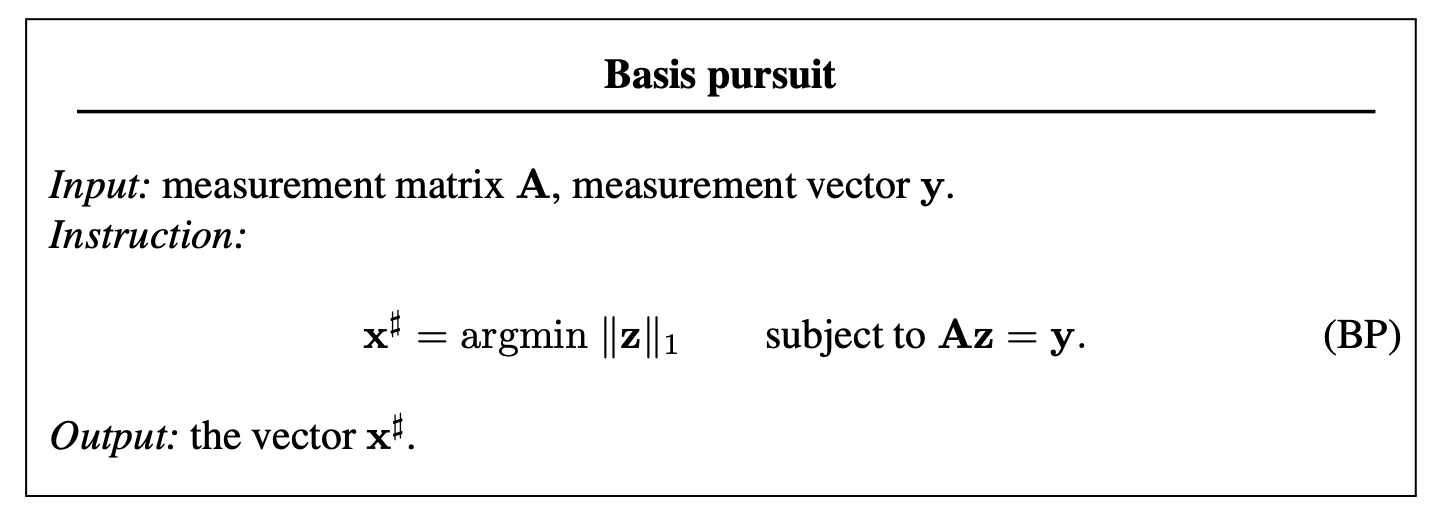
\includegraphics[width=\textwidth]{bp.png}
\end{figure}
基追踪问题可以转换为线性规划问题。
\begin{equation}
    \min _{x,u} \sum_i u_i \quad \text { subject to } \begin{cases}
    x_i-u_i  \leq 0 \\
    -x_i-u_i  \leq 0,\\
    A x  =b
    \end{cases}
\end{equation}
进而用下述算法求解。\par
\begin{figure}[!htbp]
    \centering
    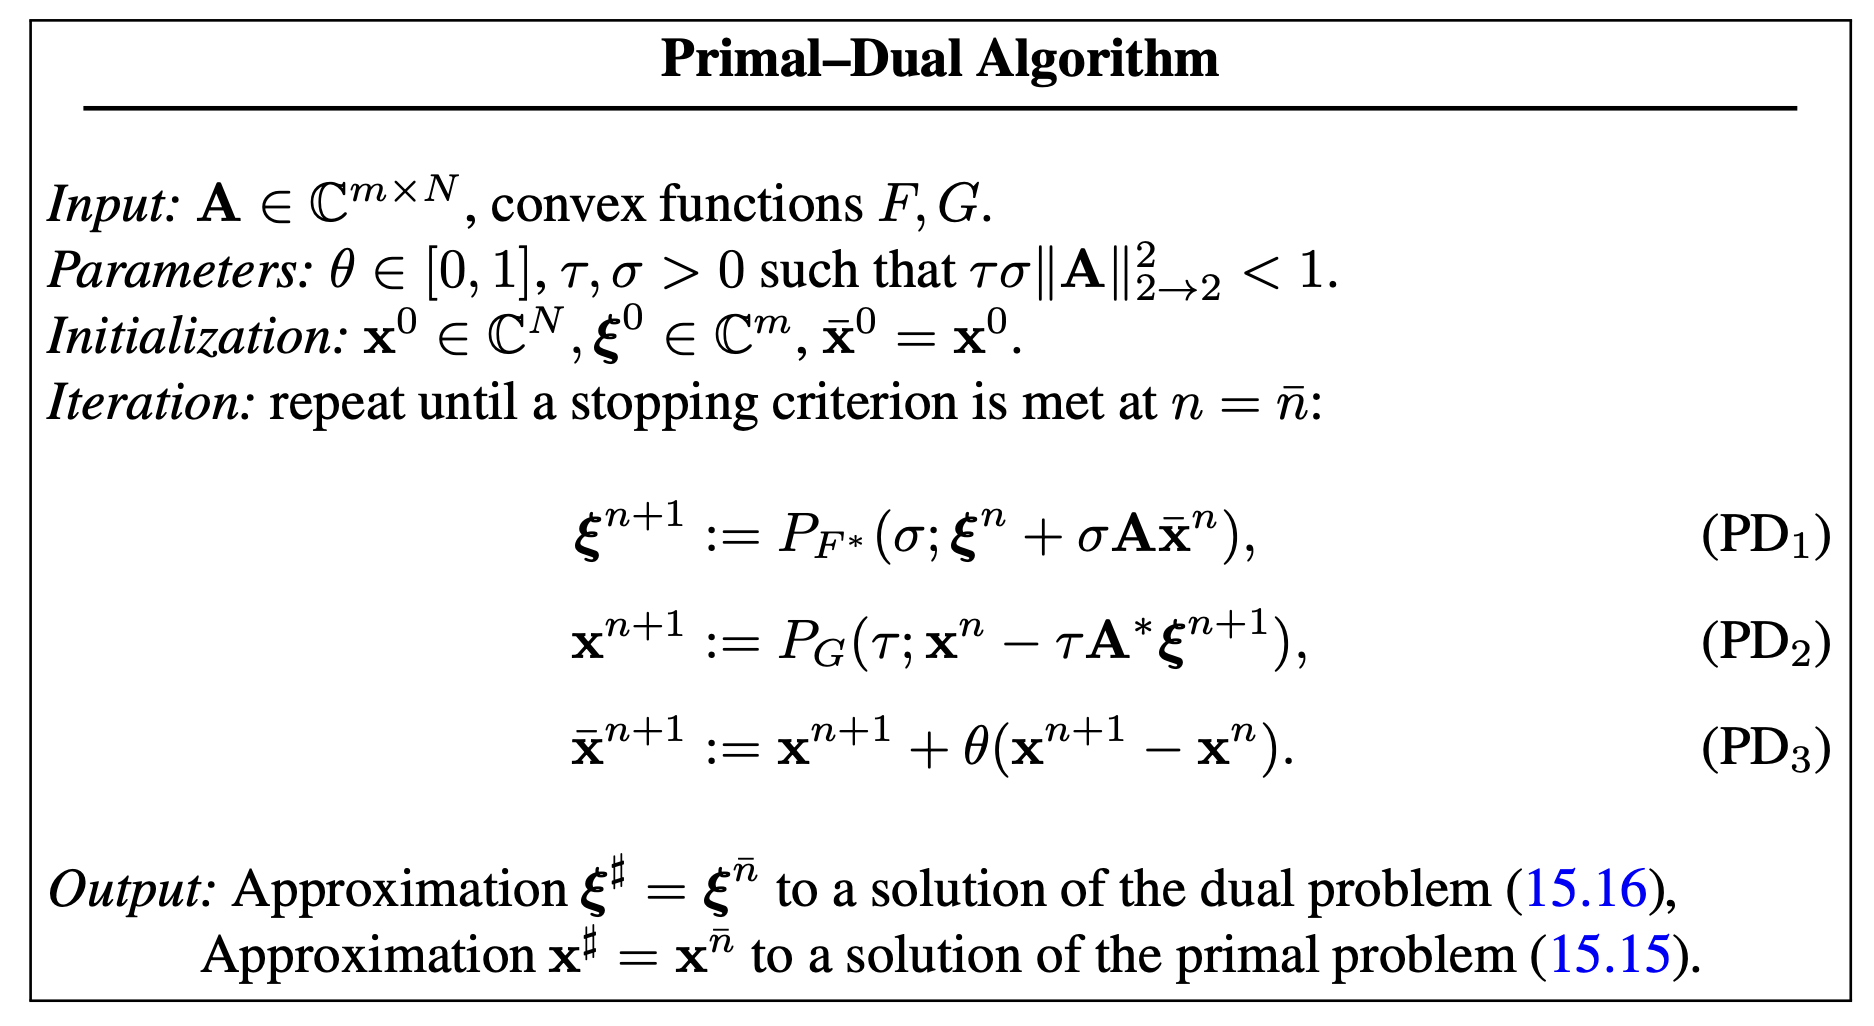
\includegraphics[width=\textwidth]{pda.png}
\end{figure}
下面是采用贪心策略的启发式算法,并不一定能收敛到最优解,首先是最经典的正交追踪。\par
\begin{figure}[!htbp]
    \centering
    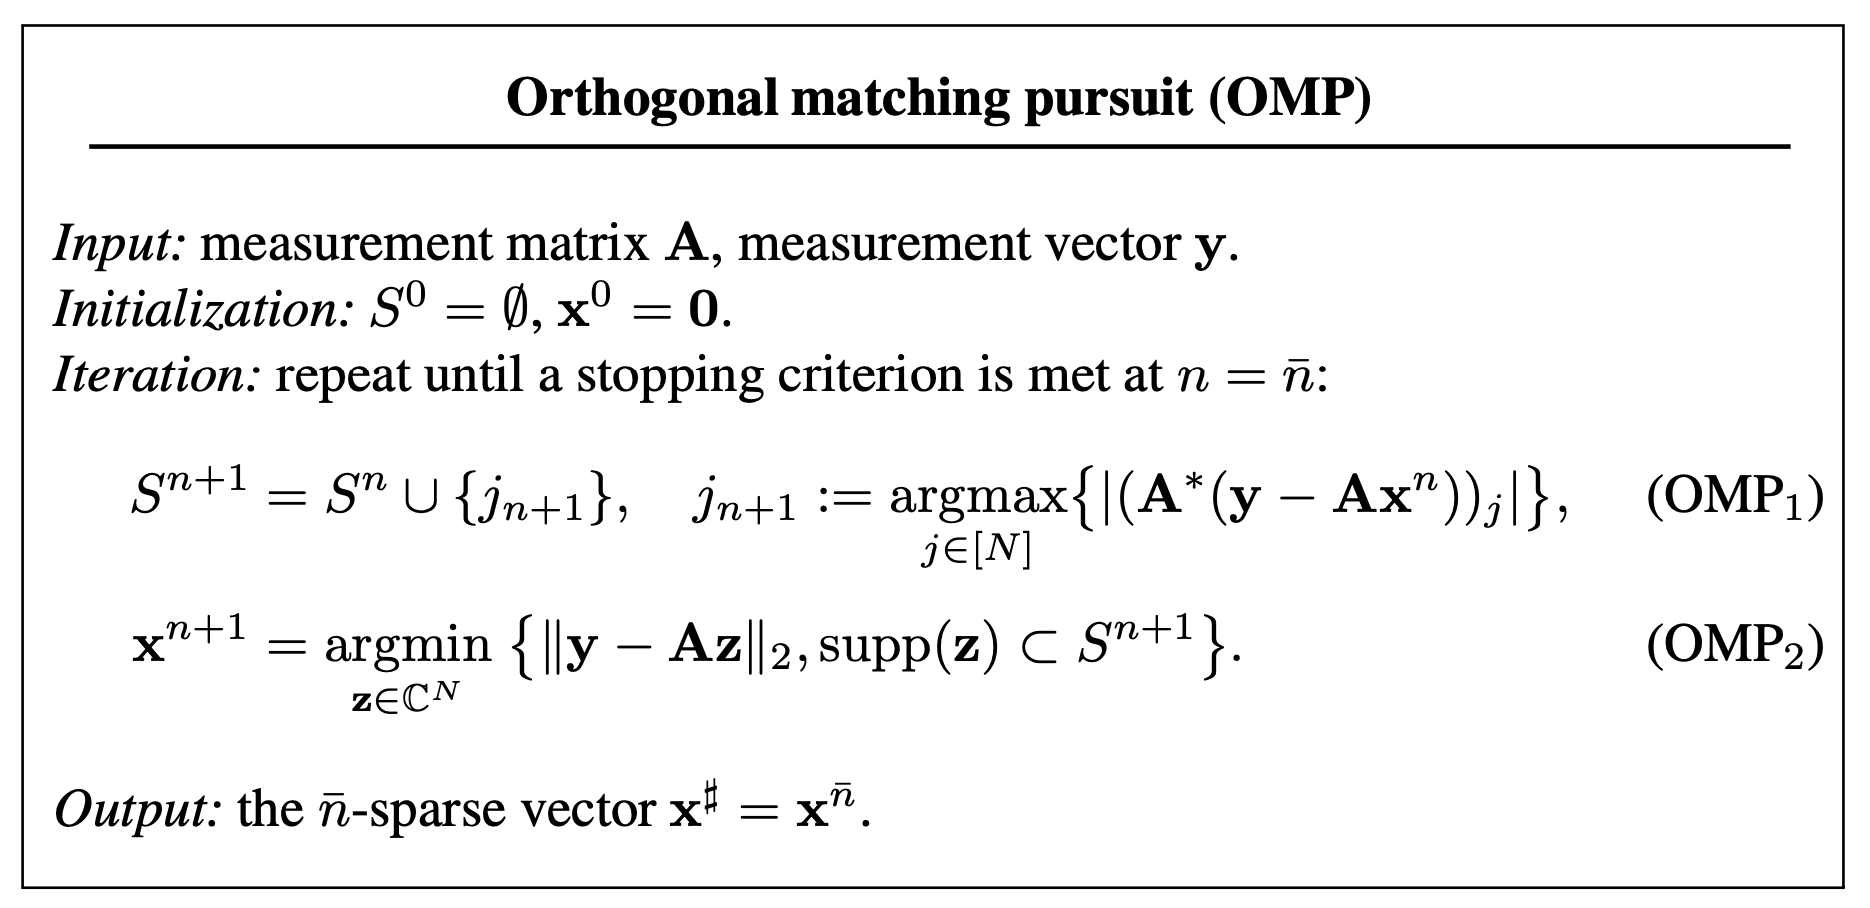
\includegraphics[width=\textwidth]{omp.png}
\end{figure}
下面的引理指出$\underset{j \in[N]}{\operatorname{argmax}}\left\{\left|\left(\mathbf{A}^*\left(\mathbf{y}-\mathbf{A} \mathbf{x}^n\right)\right)_j\right|\right\}$
确实是一个好的贪心策略。
\begin{lemma}
    令$\mathbf{A} \in \mathbb{C}^{m \times N}$是列归一化矩阵,给定的$S \subset[N]$,$\mathbf{v}$支撑在$S$上,并且
    $j \in[N]$,如果
    \begin{equation}
        \mathbf{w}:=\underset{\mathbf{z} \in \mathbb{C}^N}{\operatorname{argmin}}\left\{\|\mathbf{y}-\mathbf{A z}\|_2,\operatorname{supp}(\mathbf{z}) \subset S \cup\{j\}\right\}
    \end{equation}
    那么有
    \begin{equation}
        \|\mathbf{y}-\mathbf{A} \mathbf{w}\|_2^2 \leq\|\mathbf{y}-\mathbf{A v}\|_2^2-\left|\left(\mathbf{A}^*(\mathbf{y}-\mathbf{A} \mathbf{v})\right)_j\right|^2
    \end{equation}
\end{lemma}
\begin{proof}
任取$t \in \mathbb{C}$,形如$\mathbf{v}+t \mathbf{e}_j$的向量都支撑在$S \cup\{j\}$上,并且
\begin{equation}
    \|\mathbf{y}-\mathbf{A} \mathbf{w}\|_2^2 \leq \min _{t \in \mathbb{C}}\left\|\mathbf{y}-\mathbf{A}\left(\mathbf{v}+t \mathbf{e}_j\right)\right\|_2^2
\end{equation}
设$t=\rho e^{i \theta}$,有
\begin{equation}
    \begin{aligned}
    \left\|\mathbf{y}-\mathbf{A}\left(\mathbf{v}+t \mathbf{e}_j\right)\right\|_2^2 & =\left\|\mathbf{y}-\mathbf{A v}-t \mathbf{A} \mathbf{e}_j\right\|_2^2 \\
    & =\|\mathbf{y}-\mathbf{A v}\|_2^2+|t|^2\left\|\mathbf{A} \mathbf{e}_j\right\|_2^2-2 \operatorname{Re}\left(\bar{t}\left\langle\mathbf{y}-\mathbf{A v},\mathbf{A} \mathbf{e}_j\right\rangle\right) \\
    & =\|\mathbf{y}-\mathbf{A v}\|_2^2+\rho^2-2 \operatorname{Re}\left(\rho e^{-i \theta}\left(\mathbf{A}^*(\mathbf{y}-\mathbf{A v})\right)_j\right) \\
    & \geq\|\mathbf{y}-\mathbf{A v}\|_2^2+\rho^2-2 \rho\left|\left(\mathbf{A}^*(\mathbf{y}-\mathbf{A} \mathbf{v})\right)_j\right|
    \end{aligned}
\end{equation}
最后一式在$\rho=\left|\left(\mathbf{A}^*(\mathbf{y}-\mathbf{A} \mathbf{u})\right)_j\right|$时取最小,即
\begin{equation}
    \min _{t \in \mathbb{C}}\left\|\mathbf{y}-\mathbf{A}\left(\mathbf{v}+t \mathbf{e}_j\right)\right\|_2^2=\|\mathbf{y}-\mathbf{A v}\|_2^2-\left|\left(\mathbf{A}^*(\mathbf{y}-\mathbf{A} \mathbf{u})\right)_j\right|^2
\end{equation}
\end{proof}
正交匹配追踪算法有一个问题,一旦选择了不正确的索引,它就会保留下去,在$s$次迭代内没有办法修正。下面的CoSaMP算法增加了迭代次数,
并且采用了更有意义的索引。设$\mathbf{z} \in \mathbb{C}^N$
\begin{equation}
    L_s(\mathbf{z}):=s\text{个最大绝对条目的索引集}
\end{equation}
\begin{equation}
    H_s(\mathbf{z}):=\mathbf{z}_{L_s(\mathbf{z})}
\end{equation}
其中非线性算子$H_s$称为$s$阶硬阈值运算符,它将保留绝对值最大的前$s$项,并将其他项置为0。\par
\begin{figure}[!htbp]
    \centering
    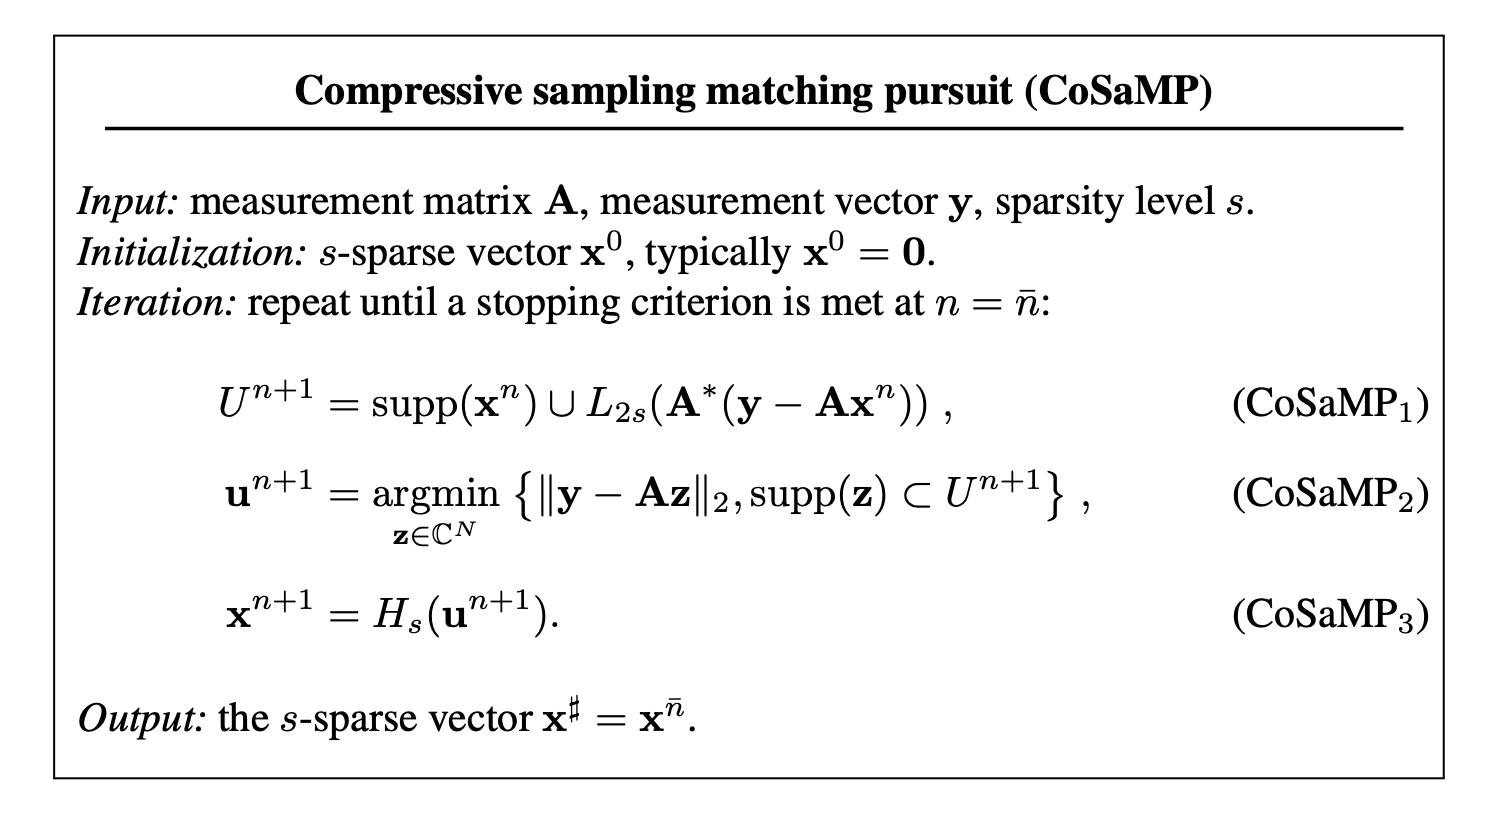
\includegraphics[width=\textwidth]{cosa.png}
\end{figure}
通过硬阈值的引入,可以将基追踪法的选取数量放宽,转变成基阈值法。\par
\begin{figure}[!htbp]
    \centering
    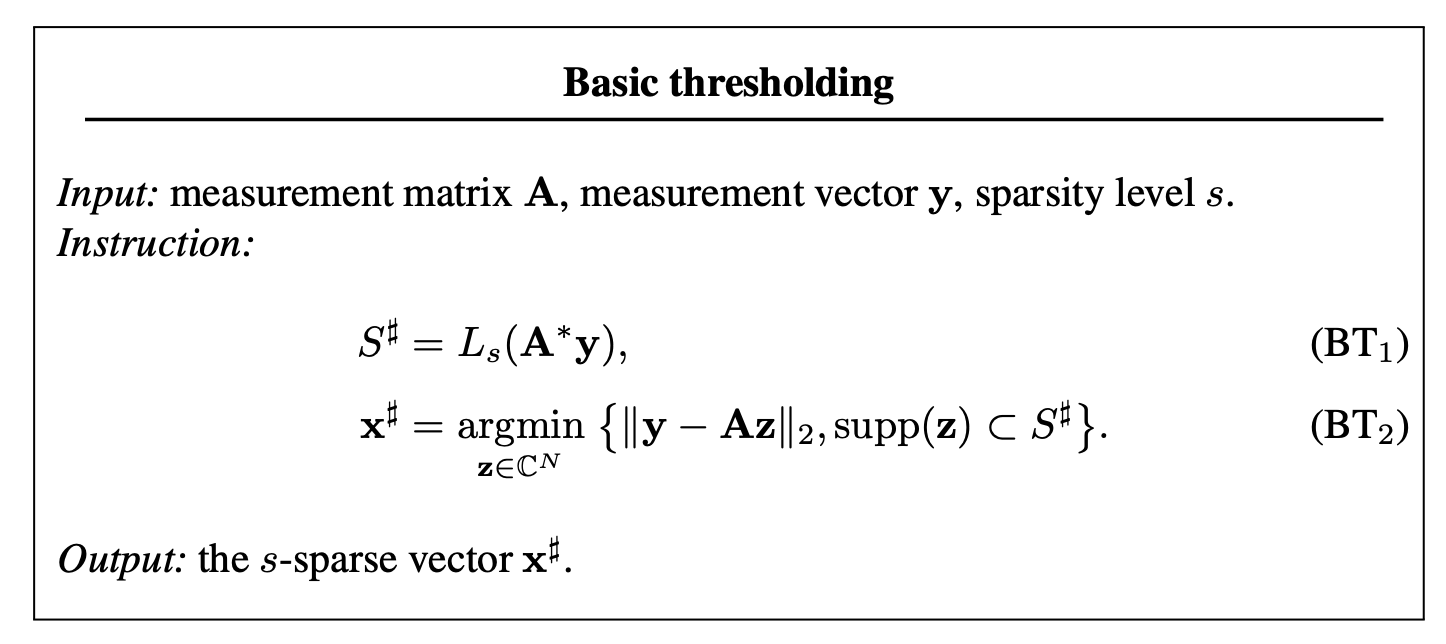
\includegraphics[width=\textwidth]{bt.png}
\end{figure}
阈值法有一个重要的性质。
\begin{proposition}
    向量可被阈值法还原的充要条件是
    \begin{equation}
        \min _{j \in S}\left|\left(\mathbf{A}^* \mathbf{y}\right)_j\right|>\max _{\ell \in \bar{S}}\left|\left(\mathbf{A}^* \mathbf{y}\right)_{\ell}\right|
    \end{equation}
\end{proposition}
接下来是阈值法的两个变种。
\begin{figure}[!htbp]
    \centering
    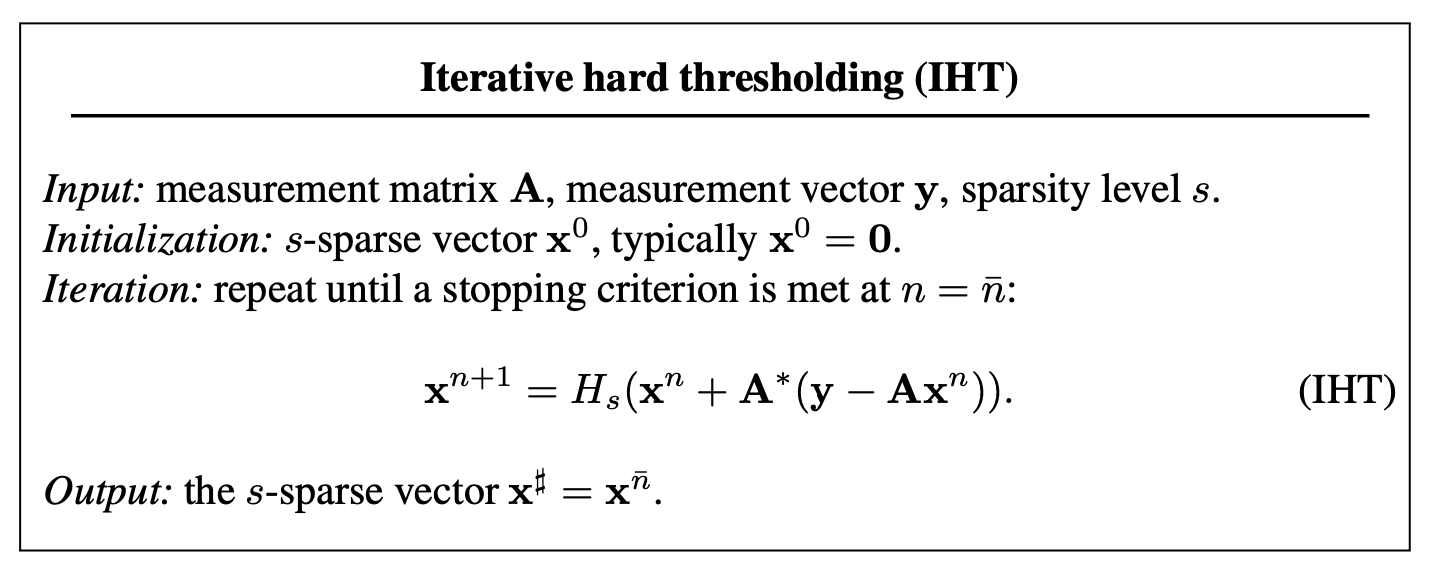
\includegraphics[width=\textwidth]{iht.png}
\end{figure}
\begin{figure}[!htbp]
    \centering
    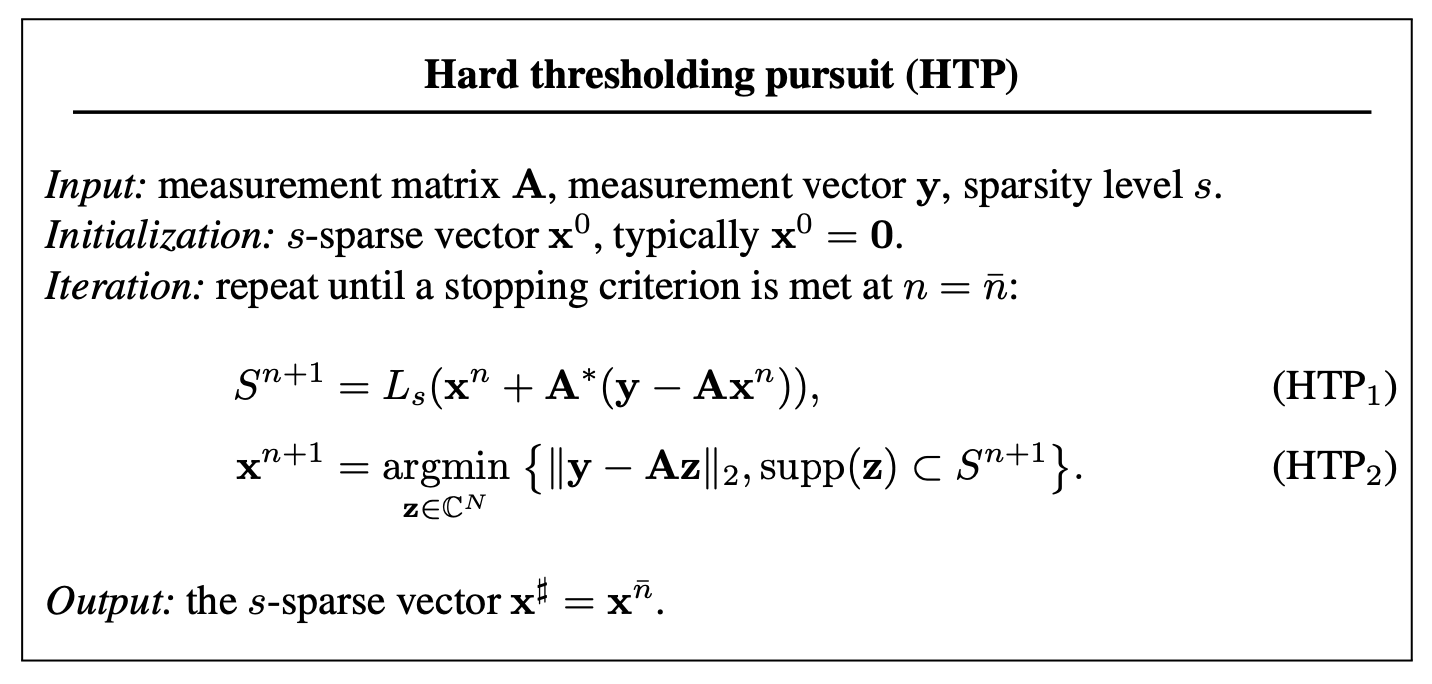
\includegraphics[width=\textwidth]{htp.png}
\end{figure}
\section{小结}